\documentclass[12pt]{article}
%%---------------------------------------------------------------------
% packages
% geometry
\usepackage{geometry}
% font
\usepackage{fontspec}
\defaultfontfeatures{Mapping=tex-text}  %%如果没有它,会有一些 tex 特殊字符无法正常使用,比如连字符。
\usepackage{xunicode,xltxtra}
\usepackage[BoldFont,SlantFont,CJKnumber,CJKchecksingle]{xeCJK}  % \CJKnumber{12345}: 一万二千三百四十五
\usepackage{CJKfntef}  %%实现对汉字加点、下划线等。
\usepackage{pifont}  % \ding{}
% math
\usepackage{amsmath,amsfonts,amssymb}
% color
\usepackage{color}
\usepackage{xcolor}
\definecolor{EYE}{RGB}{199,237,204}
\definecolor{FLY}{RGB}{128,0,128}
\definecolor{ZHY}{RGB}{139,0,255}
% graphics
\usepackage[americaninductors,europeanresistors]{circuitikz}
\usepackage{tikz}
\usetikzlibrary{positioning,arrows,shadows,shapes,calc,mindmap,trees,backgrounds}  % placements=positioning
\usepackage{graphicx}  % \includegraphics[]{}
\usepackage{subfigure}  %%图形或表格并排排列
% table
\usepackage{colortbl,dcolumn}  %% 彩色表格
\usepackage{multirow}
\usepackage{multicol}
\usepackage{booktabs}
% code
\usepackage{fancyvrb}
\usepackage{listings}
% title
\usepackage{titlesec}
% head/foot
\usepackage{fancyhdr}
% ref
\usepackage{hyperref} %生成可链接目录
% pagecolor
\usepackage[pagecolor={EYE}]{pagecolor}
% tightly-packed lists
\usepackage{mdwlist}
\usepackage{verbatim}%comment命令的注释包
\usepackage{styles/iplouccfg}
\usepackage{styles/zhfontcfg}
\usepackage{styles/iplouclistings}
\usepackage{indentfirst}
\usepackage{mathrsfs} %一些特殊数学符号
\usepackage{extarrows}%添加上下可加文字的长等号
%%---------------------------------------------------------------------
% settings
% geometry
\geometry{left=2cm,right=1cm,top=2cm,bottom=2cm}  %设置 上、左、下、右 页边距
\linespread{1.5} %行间距
% font
\setCJKmainfont{Adobe Kaiti Std}
%\setmainfont[BoldFont=Adobe Garamond Pro Bold]{Apple Garamond}  % 英文字体
%\setmainfont[BoldFont=Adobe Garamond Pro Bold,SmallCapsFont=Apple Garamond,SmallCapsFeatures={Scale=0.7}]{Apple Garamond}  %%苹果字体没有SmallCaps
\setCJKmonofont{Adobe Fangsong Std}
% graphics
\graphicspath{{figures/}}
\tikzset{
    % Define standard arrow tip
    >=stealth',
    % Define style for boxes
    punkt/.style={
           rectangle,
           rounded corners,
           draw=black, very thick,
           text width=6.5em,
           minimum height=2em,
           text centered},
    % Define arrow style
    pil/.style={
           ->,
           thick,
           shorten <=2pt,
           shorten >=2pt,},
    % Define style for FlyZhyBall
    FlyZhyBall/.style={
      circle,
      minimum size=6mm,
      inner sep=0.5pt,
      ball color=red!50!blue,
      text=white,},
    % Define style for FlyZhyRectangle
    FlyZhyRectangle/.style={
      rectangle,
      rounded corners,
      minimum size=6mm,
      ball color=red!50!blue,
      text=white,},
    % Define style for zhyfly
    zhyfly/.style={
      rectangle,
      rounded corners,
      minimum size=6mm,
      ball color=red!25!blue,
      text=white,},
    % Define style for new rectangle
    nrectangle/.style={
      rectangle,
      draw=#1!50,
      fill=#1!20,
      minimum size=5mm,
      inner sep=0.1pt,}
}
\ctikzset{
  bipoles/length=.8cm
}
% code
\lstnewenvironment{VHDLcode}[1][]{%
  \lstset{
    basicstyle=\footnotesize\ttfamily\color{black},%
    columns=flexible,%
    framexleftmargin=.7mm,frame=shadowbox,%
    rulesepcolor=\color{blue},%
%    frame=single,%
    backgroundcolor=\color{yellow!20},%
    xleftmargin=1.2\fboxsep,%
    xrightmargin=.7\fboxsep,%
    numbers=left,numberstyle=\tiny\color{blue},%
    numberblanklines=false,numbersep=7pt,%
    language=VHDL%
    }\lstset{#1}}{}
\lstnewenvironment{VHDLmiddle}[1][]{%
  \lstset{
    basicstyle=\scriptsize\ttfamily\color{black},%
    columns=flexible,%
    framexleftmargin=.7mm,frame=shadowbox,%
    rulesepcolor=\color{blue},%
%    frame=single,%
    backgroundcolor=\color{yellow!20},%
    xleftmargin=1.2\fboxsep,%
    xrightmargin=.7\fboxsep,%
    numbers=left,numberstyle=\tiny\color{blue},%
    numberblanklines=false,numbersep=7pt,%
    language=VHDL%
    }\lstset{#1}}{}
\lstnewenvironment{VHDLsmall}[1][]{%
  \lstset{
    basicstyle=\tiny\ttfamily\color{black},%
    columns=flexible,%
    framexleftmargin=.7mm,frame=shadowbox,%
    rulesepcolor=\color{blue},%
%    frame=single,%
    backgroundcolor=\color{yellow!20},%
    xleftmargin=1.2\fboxsep,%
    xrightmargin=.7\fboxsep,%
    numbers=left,numberstyle=\tiny\color{blue},%
    numberblanklines=false,numbersep=7pt,%
    language=VHDL%
    }\lstset{#1}}{}
% pdf
\hypersetup{pdfauthor={Haiyong Zheng},%
            pdftitle={Title},%
            CJKbookmarks=true,%
            bookmarksnumbered=true,%
            bookmarksopen=false,%
            plainpages=false,%
            colorlinks=true,%
            citecolor=green,%
            filecolor=magenta,%
            linkcolor=cyan,%red(default)
            urlcolor=cyan}
% section
%http://tex.stackexchange.com/questions/34288/how-to-place-a-shaded-box-around-a-section-label-and-name
\newcommand\titlebar{%
\tikz[baseline,trim left=3.1cm,trim right=3cm] {
    \fill [cyan!25] (2.5cm,-1ex) rectangle (\textwidth+3.1cm,2.5ex);
    \node [
        fill=cyan!60!white,
        anchor= base east,
        rounded rectangle,
        minimum height=3.5ex] at (3cm,0) {
        \textbf{\thesection.}
    };
}%
}
\graphicspath{{figures/}}         %% 图片路径. 本文的图片都放在这个文件夹里了.
\titleformat{\section}{\Large\bf\color{blue}}{\titlebar}{0.1cm}{}
% head/foot
\setlength{\headheight}{15pt}
\pagestyle{fancy}
\fancyhf{}
\numberwithin{equation}{section}%%公式与章节关联
%\lhead{\color{black!50!green}2014年秋季学期}
\chead{\color{black!50!green}Digital Image Processing}
%\rhead{\color{black!50!green}通信电子电路}
\lfoot{\color{blue!50!green}常琳}
%\cfoot{\color{blue!50!green}\href{http://vision.ouc.edu.cn/~zhenghaiyong}{CVBIOUC}}
\rfoot{\color{blue!50!green}$\cdot$\ \thepage\ $\cdot$}
\renewcommand{\headrulewidth}{0.4pt}
\renewcommand{\footrulewidth}{0.4pt}

%%---------------------------------------------------------------------
\begin{document}
%%---------------------------------------------------------------------
%%---------------------------------------------------------------------
% \titlepage
\title{\vspace{-2em}Computer Vision week1\vspace{-0.7em}}
\author{常琳}
\date{\vspace{-0.7em}2016年3月-\vspace{-0.7em}}
%%---------------------------------------------------------------------
\maketitle\thispagestyle{fancy}
%%---------------------------------------------------------------------
\maketitle
\tableofcontents 
%----------------------------------------------------------------------
\section{SIFT}

SIFT(Scale-invariant feature transform)是一种检测局部特征的算法。 该算法通过求一幅图中的特征点(interest points,or corner points)及其有关scale 和 orientation 的描述子得到特征并进行图像特征点匹配。
SIFT特征不只具有尺度不变性,即使改变旋转角度,图像亮度或拍摄视角,仍然能够得到好的检测效果



\subsection{构建尺度空间}

尺度空间理论目的是模拟图像数据的多尺度特征,搜索所有尺度上的图像位置。通过高斯微分函数来识别潜在的对于尺度和旋转不变的兴趣点。

1)尺度空间的表示

SIFT算法是在不同的尺度空间上查找关键点,尺度空间的获取需要使用高斯模糊来实现。一个图像的尺度空间$L(x,y,\sigma)$定义为一个变化尺度的高斯函数$G(x,y,\sigma)$与原图像$I(x,y)$的卷积。

\begin{equation}
L(x,y,\sigma)=G(x,y,\sigma)*I(x,y)
\end{equation}

\begin{equation}
G(x,y,\sigma)=\frac{1}{2\pi \sigma^{2}}e^{-\frac{(x-m/2)^{2}+(y-n/2)^{2}}{2\sigma^{2}}}
\end{equation}

$m,n$是高斯模板大小,$(x,y)$是空间坐标,$\sigma$是尺度空间因子,其大小决定图像的模糊(平滑)程度。为了有效的在尺度空间检测到稳定的关键点,提出了高斯差分尺度空间(Different of Gaussian scale-space, DOG scale-space)。利用不同尺度的高斯差分核与图像卷积生成。

\begin{equation}
D(x,y,\sigma)=(G(x,y,k\sigma)-G(x,y,\sigma))*I(x,y)=L(x,y,k\sigma)-L(x,y,\sigma)
\end{equation}

2)高斯金字塔的构建

图像的金字塔模型是指将原始图像不断进行降阶采样,得到一系列大小不一的图像,由大到小,从下到上构成的塔状模型。每次降采样所得到的新图像为金字塔的一层,此时每层有一张图像,每个金字塔共n层,层数由图像的原始大小和塔顶图像的大小共同决定。

为了让尺度体现其连续性(scale-invariant,也就是在任何尺度都能够有对应的特征点),高斯金字塔在简单降采样的基础上加了高斯滤波,将图像金字塔每层的一张图像使用不同参数做高斯滤波,使得金字塔的每层含有多张高斯模糊图像,将金字塔每层多张图像合称为一组(Octave也称为子八度)。同一个octave中的图片尺寸(大小)相同,但尺度(模糊程度)不同;不同的octave层中图片的尺寸也不同,因为后面每个octave层的底层图像为上一个octave中倒数第三张图像隔点采样的结果,即原图的1/4(长宽分别减半)。在进行高斯模糊时,sift的高斯模板大小始终是不变的,只是在不同的octave之间改变图片的大小。

在实际计算时,使用高斯金字塔每组中相邻上下两层图像相减,得到高斯差分图像。如图\ref{dog}所示。

\begin{figure}[!ht]
  \centering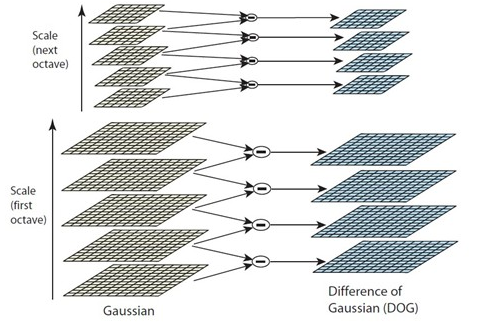
\includegraphics[width=3.5in]{dog.png}
  \caption{金字塔}
 \label{dog}
  \end{figure}

在检测极值点前对原始图像的高斯平滑以致图像丢失高频信息,所以 Lowe 建议在建立尺度空间前首先对原始图像长宽扩展一倍,以保留原始图像信息,增加特征点数量。

\subsection{检测DOG尺度空间极值点}

将检测点和它同尺度的8个相邻点和上下相邻尺度对应的9×2个点共26个点比较,以确保在尺度空间和二维图像空间都检测到极值点。 一个点如果在DOG尺度空间本层以及上下两层的26个领域中是最大或最小值时,就认为该点是图像在该尺度下的一个特征


为了在每组中检测S个尺度的极值点,则DOG金字塔每组需S+2层图像,而DOG金字塔由高斯金字塔相邻两层相减得到,则高斯金字塔每组需S+3层图像,实际计算时S在3到5之间。




\subsection{精确定位极值点}

通过拟合三维二次函数以精确确定关键点的位置和尺度(达到亚像素精度),同时去除低对比度的关键点和不稳定的边缘响应点,以增强匹配稳定性,提高抗噪声能力。

1)关键点的精确定位

关键点的尺度坐标:

\begin{equation}
\sigma(o,s)=\sigma_{0}2^{o+\frac{s}{S}}  \quad o=0,1,\ldots,O-1, s=0,\ldots,S+2
\end{equation}

$\sigma_{0}$是基准层尺度,$o$为octave的索引,$s$为组内层的索引,$O,S$分别为组数和组内层数。

计算某一层图像的尺度:

\begin{equation}
\sigma\__{oct}(s)=\sigma_{0}2^{\frac{s}{S}}  \quad s=0,\ldots,S+2
\end{equation}


空间尺度函数泰勒展开式如下:

\begin{equation}
D(X)=D(X)+\frac{\partial D^{T}}{\partial X}X+\frac{1}{2}X^{T}\frac{\partial ^{2}D}{\partial X^{2}}X
\end{equation}

其中,$X=(x,y,\sigma)^{T}$

对上式求导,并令其为0,得到极值点的偏移量为:

\begin{equation}
\^{X}=-\frac{\partial ^{2}D^{-1}}{\partial X^{2}}\frac{\partial D}{\partial X}
\end{equation}

对应极值点处方程的值,只取前两项可得:

\begin{equation}
D(\^{X})=D+\frac{\partial D^{T}}{\partial {X}}\^{X}
\end{equation}
(应该是个减号吧?)

$\left|D(X)\right|$过小的点易受噪声的干扰而变得不稳定,所以将$\left|D(X)\right|$小于某个经验值的极值点删除,Lowe论文中使用0.03。 在这一过程中获得特征点的精确位置(原位置加拟合偏移量)以及尺度。

2)消除边缘响应

一个定义不好的高斯差分算子的极值在横跨边缘的地方有较大的主曲率,而在垂直边缘的方向有较小的主曲率。DOG算子会产生较强的边缘响应,需要剔除不稳定的边缘响应点。获取特征点处的Hessian矩阵,主曲率通过一个$2*2$的Hessian矩阵H求出:

$H=$
\begin{gather*}
\begin{bmatrix}
D_{xx} & D_{xy}\\
D_{xy} & D_{yy}
\end{bmatrix}
\end{gather*}
导数由采样点相邻差估计得到。

H的特征值$\alpha$ 和$\beta$代表$x$和$y$方向的梯度,令

\begin{equation}
Tr(H)=D_{xx}+D_{yy}=\alpha +\beta \\
Det(H)=D_{xx}D_{yy}-(D_{xy})^{2}=\alpha \beta
\end{equation}

分别表示矩阵H对角线元素之和、矩阵H的行列式。假设$\alpha$ 是较大的特征值,$\beta$是较小的特征值,令$\alpha =r\beta$,则
\begin{equation}
\frac{Tr(H)^{2}}{Det(H)}=\frac{(\alpha_ \beta)^{2}}{\alpha \beta}=\frac{(r\beta +\beta)^{2}}{r\beta^{2}}=\frac{(r+1)^{2}}{r}
\end{equation}

D的主曲率和H的特征值$\alpha ,\beta$成正比,公式$(r+1)^{2}/r$的值在两个特征值相等时最小,随着r的增大而增大。值越大,说明两个特征值的比值越大,即在某一个方向的梯度值越大,而在另一个方向的梯度值越小,而边缘恰恰就是这种情况。所以为了剔除边缘响应点,需要让该比值小于一定的阈值,因此只需检测
\begin{equation}
\frac{Tr(H)^{2}}{Det(H)}<\frac{(r+1)^{2}}{r}
\end{equation}
Lowe的文章中取$r=10$,上式成立时将关键点保留,反之剔除。

\subsection{关键点方向匹配}

对上面提取的每个关键点,围绕该点选择一个窗口(圆形区域,建议半径$3*1.5\sigma\_ _{oct}$),窗口内各采样点的梯度方向构成一个方向直方图,根据直方图的峰值确定关键点的方向。

L所用的尺度为关键点所在的尺度。按尺度采样对于窗口内的每个采样点$(x,y)$,其梯度向量的幅度和方向$m(x,y)$,$\theta(x,y)$公式为:

\begin{equation}
m(x,y)=\sqrt{(L(x+1,y)-L(x-1,y))^{2}+(L(x,y+1)-L(x,y-1))^{2}}\\
\end{equation}

\begin{equation}
\theta =\tan^{-1}((L(x,y+1)-L(x,y-1))/(L(x+1,y)-L(x-1,y)))
\end{equation}

做一个梯度方向的直方图,范围是$0-360$度,其中每10度一个柱,总共36个柱,每个采样点按照其梯度方向$\theta(x,y)$加权统计到直方图(圆形高斯加权函数,标准偏差为$\sigma=1.5\sigma\_ _{oct}$),权值为幅度$m(x,y)$和贡献因子的乘积。贡献因子是采样点到关键点(窗口中心)距离的量度(就是类似那个高斯函数的式子),距离越大,贡献因子越小。直方图的峰值代表了该关键点处邻域梯度的主方向。如图\ref{fangxiang}
\begin{figure}[!ht]
  \centering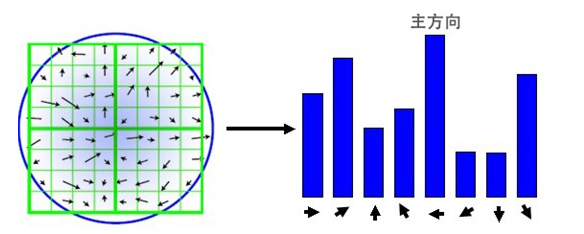
\includegraphics[width=3in]{guanjiandian_fangxiang_zhifangtu.png}
  \caption{关键点方向直方图}
 \label{fangxiang}
  \end{figure}

对于多峰值(幅值大于峰值的80\%)情形,在同一个位置和尺度会产生多个具有不同方向的关键点。用每个峰值和左右两个幅值拟合二次曲线,以定位峰值的实际位置(抛物线的最高点)。

\subsection{关键点描述子的生成}
首先将坐标轴旋转为关键点的方向,以确保旋转不变性。计算keypoint周围的$16*16$的window中每一个像素的梯度,每个小格代表关键点邻域所在尺度空间的一个像素,利用公式求得每个像素的梯度幅值与梯度方向,箭头方向代表该像素的梯度方向,箭头长度代表梯度模值,然后用高斯窗口对其进行加权运算。然后在每$4*4$的小块上计算8个方向的梯度方向直方图(作者建议),绘制每个梯度方向的累加值,即可形成一个种子点,如图右部分示。这样就可以对每个feature形成一个$4*4*8=128$维的描述子,每一维都可以表示$4*4$个格子中一个的scale/orientation. 将这个向量归一化之后,就进一步去除了光照的影响。

1)确定计算描述子所需的图像区域

对梯度的求取应在特征点对应的高斯图像上进行,将关键点附近的邻域划分为$d*d(d=4)$个子区域,每个子区域作为一个种子点,每个种子点有八个方向,每个子区域的大小与关键点方向分配时相同,即每个区域有$3\sigma\_ _{oct}$个子像素,为每个区域分配边长为$3\sigma\_ _{oct}$的矩形区域进行采样(实际用边长为$\sqrt{3\sigma\_ _{oct}}$)。考虑到实际计算时,需要采用双线性插值,所需图像窗口边长为$3\sigma\_ _{oct}*(d+1)$。计算所需的图像区域半径为:
\begin{equation}
radius=\frac{3\sigma\_ _{oct}*\sqrt{2}*(d+1)}{2} \quad (d=4)
\end{equation}

2)将坐标旋转为关键点的方向,以确保旋转不变性
\begin{figure}
  \centering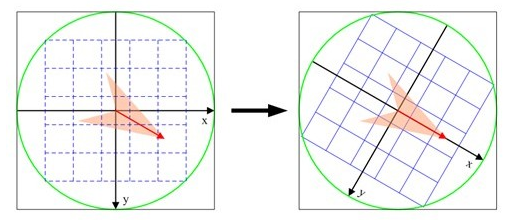
\includegraphics[width=3.5in]{zuobiaozhouxuanzhuan.png}
  \caption{坐标轴旋转}
 \label{zuobiaoxuanzhuan}
  \end{figure}

旋转后邻域内的新坐标为:

\begin{gather*}
\begin{bmatrix}
x'\\
y'
\end{bmatrix}
=
\begin{bmatrix}
\cos\theta & -\sin\theta \\
\sin\theta & \cos\theta
\end{bmatrix}
\begin{bmatrix}
x\\
y
\end{bmatrix}
\end{gather*}

3)将邻域内的采样点分配到对应的子区域内,将子区域内的梯度值分配到8个方向上,计算权值。(因为旋转了,所以要重新采样再分配?)

旋转后的采样坐标在半径为radius的圆内被分配到$d*d$的子区域,计算子区域的采样点的梯度和方向,分配到八个方向上。分配后的下标:

\begin{gather*}
\begin{bmatrix}
x"\\
y"
\end{bmatrix}
=
\frac{1}{3\sigma\_ _{oct}}
\begin{bmatrix}
x'\\
y'
\end{bmatrix}
\end{gather*}
$+\frac{d}{2}$

Lowe建议子区域的像素梯度大小按$\sigma=0.5d$的高斯加权计算,即

\begin{equation}
w=m(a+x,b+y)*e^{-\frac{(x')^{2}+(y')^{2}}{2x(0.5d)^{2}}}
\end{equation}

$a,b$为关键点在高斯金字塔图像中的位置坐标。

4)插值计算每个种子点八个方向的梯度
\begin{figure}
  \centering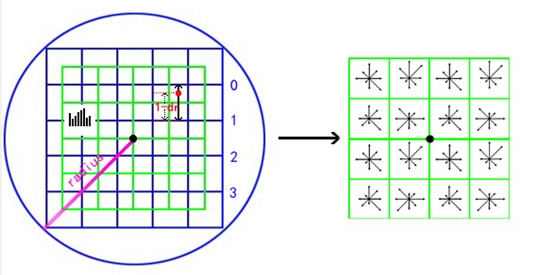
\includegraphics[width=3.5in]{miaoshuzi.png}
  \caption{描述子梯度直方图}
 \label{miaoshuzi}
  \end{figure}

如图\ref{miaoshuzi}所示,将所得采样点在子区域中的下标$(x",y")$(蓝色窗口内红色点)线性插值,计算其对每个种子点的贡献。如图中红色的点,落在第0行和第1行之间,对这两行都有贡献。对第0行第3列种子点的贡献因子为$dr$,对第1行第3列的贡献因子为$1-dr$,对临近两列的贡献因子为$dc$和$1-dc$对邻近两个方向贡献因子为$do$,$1-do$。最终累加在每个方向上的梯度大小为:

\begin{equation}
weight=w*dr^{k}*(1-dr)^{1-k}*dc^{m}*(1-dc)^{1-m}*do(1-do)^{1-n}
\end{equation}

其中k,m,n为0或1。

5)如上统计的$4*4*8=128$个梯度信息即为该关键点的特征向量,得到的描述子向量为$H=(h_{1},h_{2},\ldots,h_{128})$。为了去除光照变化的影响,需要对它们进行归一化处理,归一化后的特征向量为$L=(l1,l2,\ldots,l128)$,则

\begin{equation}
l_{i}=\frac{h_{i}}{\sqrt{\sum_{j=1}^{128}h_{j}}}
\end{equation}

\subsection{匹配}

采用欧式距离来作为两幅图像的关键点的相似性度量。

模板图中关键点描述子:$R_{i}=(r_{i1},r_{i2},\ldots,r_{i128})$

实时图中关键点描述子:$S_{i}=(s_{i1},s_{i2},\ldots,s_{i128})$

任意两描述子相似性度量:$d(R_{i},S_{i})=sqrt{\sum_{j=1}^{128}(r_{ij}-s_{ij})^{2}}$

配对条件:

实时图中距离$R_{i}$最近的点$S_{j}$/实时图中距离$R_{i}$的次最近点$S_{p}$<Threshold


\section{SURF}

SURF(Speeded Up Robust Features)is a robust local feature detector, first presrnted by Herbert Bayet al. in 2006. It is partly inspired by the SIFT descriptor.
\subsection{Construct scale-space}
每一层图像上使用快速 Hessian 矩阵来检测图像的极值点。
SURF中,图片的大小是一直不变的,不同Octave层的带检测图片是改变高斯模糊尺度大小得到的。算法允许尺度空间多层图像同时被处理,不需要对图像进行二次抽样。没有进行降采样。


\subsection{特征点主方向选取}
为了保持旋转不变性
sift选取特征点的主方向是采用在特征点领域内统计其梯度直方图,取直方图bin值最大的以及超过最大值80%的哪些方向作为主方向。
在surf中,是统计特征点领域内的harr小波特征。即在特征点的领域(比如半径为6s的圆内,s为该点所在的尺度)内,统计60度扇形内所有点的水平haar小波特征和垂直小波特征总和,haar小波的尺寸边长为4s,这样扇形得到了一个值。然后60度扇形以一定间隔进行旋转(5度),最后将最大值那个扇形的方向作为该特征点的主方向。

\subsection{构造特征点描述算子}
在sift中,是在特征点周围选取16*16的邻域,并把该邻域化为4×4个的小区域,每个小区域统计8个方向梯度,最后得到128维的向量作为描述子。

在surf中,是在特征点周围取一个正方形框,边长20s,方向为该特征点的主方向,然后把框分为16个子区域,每个子区域统计25个像素的水平方向和垂直方向的haar小波特征,这里的水平和垂直方向都是相对主方向而言的。该haar小波特征为水平方向值之和,水平方向绝对值之和,垂直方向之和,垂直方向绝对值之和。这样每个小区域就有4个值,所以每个特征点就是$16*4=64$维的向量。比sift少了一半,会大大加快匹配速度。

\section{LBP}

LBP就是一种局部信息,它反应的内容是每个像素与周围像素的关系。
LBP算子的基本思想是将中心像素点的灰度值设为阈值,其圆形邻域内的像素点与之作比较得到二进制码用来表述局部纹理特征,在描述纹理特征提取方面有着显著的效果.对任意的LBP算子,它的编码公式为:
\begin{equation}
LBP_{P,R}=\sum_{i=0}^{p-1}s(g_{i}-g_{c})2^{i}, s(x)= \left\{ \begin{array}{ll}
1 & \textrm{$x\geq0$}\\
0 & \textrm{$x<0$}\\
\end{array} \right.
\end{equation}

其中P表示邻域内包含的像素个数,R表示邻域半径.式中gi表示P个以中心像素gc为圆心,R为半径的圆周上的像素值,具体计算过程如图3,P8,R=1,将图3左边模板阈值化,即使各邻域像素点与中心像素做比较得到s的值,大于0s=1,小于0则s=0,得到图3中间图,确定各像素点的权重,如图3右图,计算阈值化后各像素与对应权重的点积,(将图3中间图的二进制数转化为十进制),即为LBP算子,可以用这个值来反应该区域的纹理信息.将LBP特征进行直方图统计,即统计LBP特征0~255各占的比例,就可以得到一个具有256维特征的数据.

我们:先将藻种图片大小统一一处理成64*64,再将图片划分成8*8块区域,对每个小区域进行LBP处理,再将每个小区域的直方图进行串联,得到整个图像的LBP直方图,进而获得一个1400*16384的矩阵,其中16384=8*8*256是数据维度.之后再将矩阵进行PCA降维,得到降维后的LBP特征矩阵.


%===========================================================================================================
\end{document}




 


